
%\PassOptionsToPackage{showframe}{geometry}
\documentclass[11pt,twoside,openright]{kaobook}



%\usepackage[
%    left=0.5in,
%    right=0.5in,
%    top=0.75in,
%    bottom=1.0in,
%    paperwidth=8.25in,
%    paperheight=11in,
%    bindingoffset=0.375in
%    ]{geometry}

\input{pandoc.tex}

%\usepackage[style=ieee]{biblatex}

\pretocmd\longtable{\scriptsize}{}{}
\setcounter{secnumdepth}{3}
\counterwithin*{sidenote}{chapter}


\urlstyle{same} % disable monospaced font for URLs
\hypersetup{
  pdftitle={Advanced Integrated Circuits 2025},
  pdfauthor={Carsten~Wulff},
  colorlinks=true,
  linkcolor={Maroon},
  filecolor={Maroon},
  citecolor={Blue},
  urlcolor={Blue},
  pdfcreator={}}
\usepackage{flafter}

\usepackage{longtable,booktabs,array}

\newcommand{\myfigwidth}{100mm}
\newcommand{\myfigheight}{100mm}


  \newcommand\BackgroundPic{%
\put(0,0){%
\parbox[b][\paperheight]{\paperwidth}{%
\vfill
\centering
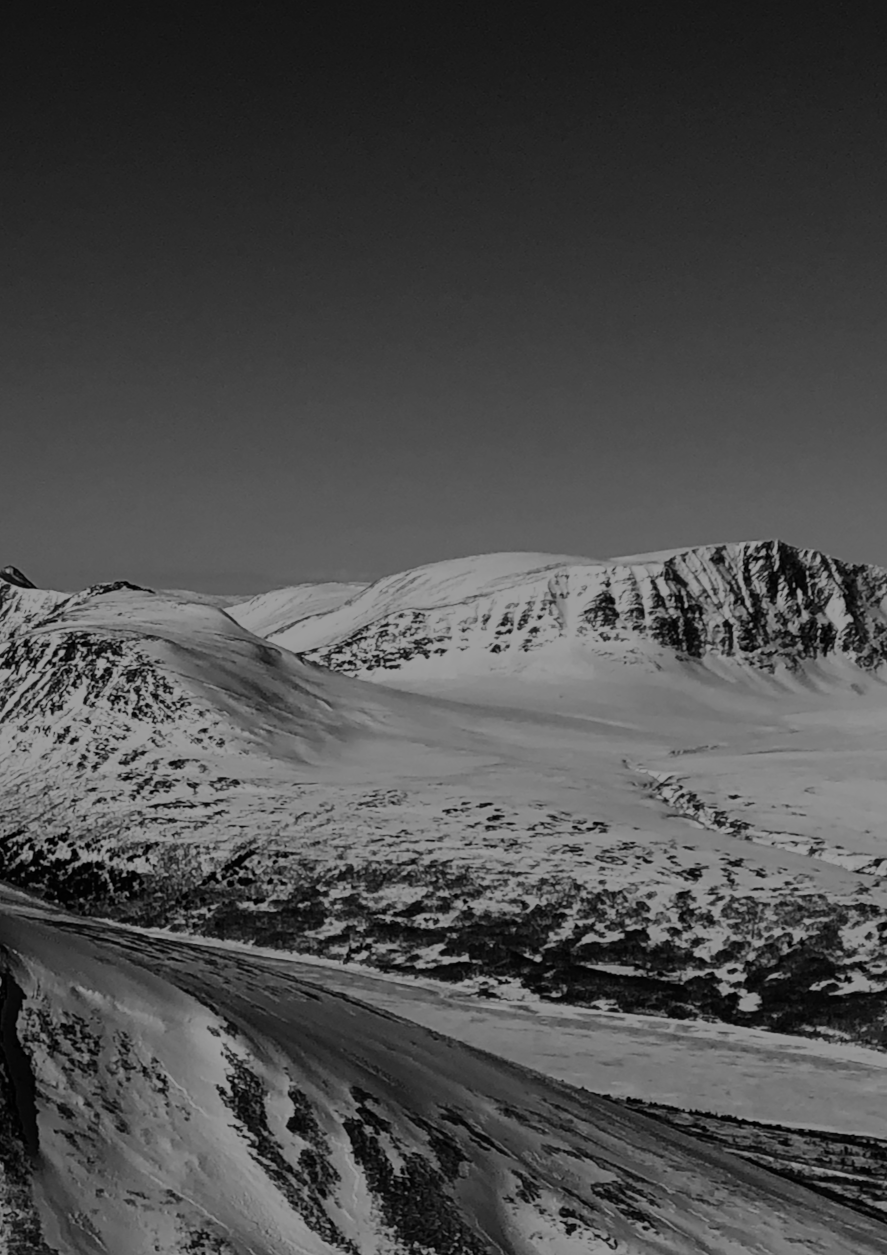
\includegraphics[width=\paperwidth,height=\paperheight,%
keepaspectratio]{background.png}%
\vfill
}}}


\title{Advanced Integrated Circuits 2025}
\author{Carsten~Wulff}
\date{}

\begin{document}

\AddToShipoutPicture*{\BackgroundPic}

\begin{titlepage} % Suppresses displaying the page number on the title page and the subsequent page counts as page 1

	\raggedleft % Right align the title page

  {
    \color{white}

	\rule{1pt}{\textheight} % Vertical line
	\hspace{0.05\textwidth} % Whitespace between the vertical line and title page text
	\parbox[b]{0.75\textwidth}{ % Paragraph box for holding the title page text, adjust the width to move the title page left or right on the page

		{\Huge\bfseries Advanced Integrated Circuits}\\[2\baselineskip] % Title
		{\large\textit{Lecture Notes 2025}}\\[4\baselineskip] % Subtitle or further description
		{\Large\textsc{Carsten Wulff}} % Author name, lower case for consistent small caps

		\vspace{0.5\textheight} % Whitespace between the title block and the publisher

    {\noindent Built on Sun Jun  8 14:07:09 CEST 2025} \\ 
 {\noindent from 025f7d2ffc08a892be68fd60ec4f5a781348431d}


		{\noindent \copyright Carsten Wulff 2025}\\[\baselineskip]
	}

  }



\end{titlepage}



{
\hypersetup{linkcolor=}
\setcounter{tocdepth}{2}
\tableofcontents
}

\bibliographystyle{IEEEtran}

\mainmatter

%\chapter{Background}
%\input{tex_intro_fiximg.tex}

\input{chapters.tex}
% \setchapterstyle{kao}
% \setchapterpreamble[u]{\margintoc}
% \chapter{Introduction}
% \input{lecture_1_-__introduction_fiximg.tex}

% %\setchapterstyle{kao}
% %\setchapterpreamble[u]{\margintoc}
% %\chapter{How to write a project report}
% %\input{how_to_write_a_project_report_fiximg.tex}

% \setchapterstyle{kao}
% \setchapterpreamble[u]{\margintoc}
% \chapter{Refresher}
% \input{a_refresher_fiximg.tex}

% \setchapterstyle{kao}
% \setchapterpreamble[u]{\margintoc}
% \chapter{Diodes}
% \input{diodes_fiximg.tex}

% \setchapterstyle{kao}
% \setchapterpreamble[u]{\margintoc}
% \chapter{Mosfets}
% \input{mosfets_fiximg.tex}

% \setchapterstyle{kao}
% \setchapterpreamble[u]{\margintoc}
% \chapter{Spice}
% \input{spice_fiximg.tex}

%  \setchapterstyle{kao}
% \setchapterpreamble[u]{\margintoc}
% \chapter{Skywater 130nm tutorial}
% \input{sky130nm_tutorial_fiximg.tex}


% \setchapterstyle{kao}
% \setchapterpreamble[u]{\margintoc}
% \chapter{ESD and IC}
% \input{lecture_2_-_ic_and_esd_fiximg.tex}

% \setchapterstyle{kao}
% \setchapterpreamble[u]{\margintoc}
% \chapter{References and bias}
% \input{lecture_3_-_references_and_bias_fiximg.tex}

% \setchapterstyle{kao}
% \setchapterpreamble[u]{\margintoc}
% \chapter{Analog frontend and filter}
% \input{lecture_4_-_analog_frontend_and_filters_fiximg.tex}

% \setchapterstyle{kao}
% \setchapterpreamble[u]{\margintoc}
% \chapter{Switched capacitor circuits}
% \input{lecture_5_-_switched-capacitor_circuits_fiximg.tex}

% \setchapterstyle{kao}
% \setchapterpreamble[u]{\margintoc}
% \chapter{Oversampling and Sigma-Delta ADCs}
% \input{lecture_6_-_oversampling_and_sigma-delta_adcs_fiximg.tex}

% \setchapterstyle{kao}
% \setchapterpreamble[u]{\margintoc}
% \chapter{Voltage Regulation}
% \input{lecture_7_-_voltage_regulation_fiximg.tex}

% \setchapterstyle{kao}
% \setchapterpreamble[u]{\margintoc}
% \chapter{Clocks and PLLs}
% \input{lecture_8_-_clocks_and_plls_fiximg.tex}

% \setchapterstyle{kao}
% \setchapterpreamble[u]{\margintoc}
% \chapter{Oscillators}
% \input{lecture_9_-_oscillators_fiximg.tex}

% \setchapterstyle{kao}
% \setchapterpreamble[u]{\margintoc}
% \chapter{Low Power Radio}
% \input{lecture_10_-_low_power_radio_fiximg.tex}

%  \setchapterstyle{kao}
% \setchapterpreamble[u]{\margintoc}
% \chapter{Analog SystemVerilog}
% \input{lecture_11_-_analog_systemverilog_fiximg.tex}

% \setchapterstyle{kao}
% \setchapterpreamble[u]{\margintoc}
% \chapter{Energy Sources}
% \input{lecture_x_-_energy_sources_fiximg.tex}

%\chapter{What I expect you to know}
%\input{what_i_expect_you_to_already_know.latex}


%\bibliographystyle{IEEEtran}
\bibliography{aic.bib}

\backmatter


\end{document}
